\documentclass[a4paper,10pt]{article}
\usepackage[left=2cm,top=2cm,right=2cm,bottom=2cm]{geometry}
\usepackage[utf8]{inputenc}
\usepackage{amsthm}
\usepackage{graphicx}
\graphicspath{ {images/} }


\newcommand{\mN}{{\mathbb N}}
\newcommand{\mZ}{{\mathbb Z}}
\newcommand{\cZ}{{\mathcal Z}}
\newcommand{\fL}{{\mathfrak L}}
\newcommand{\dst}{\displaystyle}

%opening
\title{}
\author{}
\date{}

\begin{document}

\maketitle
Carlos Gallegos\\\\
Parcial 2 \\\\
1 La corriente en un alambre produce un campo magnético 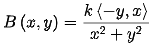
\includegraphics[scale=.4]{../campo eléctrico.png}   . Bosqueja un alambre con su campo magnético.\\\\
https://www.geogebra.org/m/re9garx5\\\\\\
2 Demuestra que 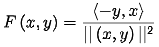
\includegraphics[scale=.4]{../conservativo.png}  es conservativo siempre que $y>0$, para ello encuentra una función potencial.\\\\
Primero buscamos una integral respecto a x de $\frac{-y}{\sqrt{x^2 + y^2}}$ la cual es $-y\cdot arsinh(\frac{x}{|y|})$. Luego respecto a y de $\frac{x}{\sqrt{x^2 + y^2}}$ la cual es $x\cdot arsinh(\frac{y}{|x|})$.Podemos tener como función potencial $-y\cdot arsinh(\frac{x}{|y|}) + x\cdot arsinh(\frac{y}{|x|})$\\\\\\
3 Si T proporciona la temperatura en el punto , el campo de velocidad para el flujo de calor está dado por  para una constante . Esto se conoce como Ley de Fourier. Utilice este campo vectorial para determinar si el calor fluye de caliente a frío o viceversa. \\\\
El signo negativo nos indica que la dirección de calor es decreciente a la temperatura. Como tenemos k positivo, sea $T1>T2$ no existe un gradiente que fluya de T2 a T1, porque k es positivo. Por lo tanto el calor fluye caliente a frío.\\\\\\
4 Podemos comprobar que la función potencial del campo F(y,x)=y,x es f(x,y)=xy, porque al derivar respecto a x nos queda y; al derivar respecto a y nos queda x.\\\\
Para probar que la función de flujo es solución de la ecuación de Laplace, es suficiente ver que si derivamos $g(x,y)= \frac{1}{2}(y^2 -x^2)$ nos queda -x(cuando es respecto a x) y nos queda y(cuando es respecto a y). Entonces, si derivamos por segunda vez nos queda cero. Por lo tanto, usando g(x,y)=u, se cumple que $\bigtriangledown u= u_{xx} + u_{yy}$ porque $0+0=0$.\\\\\\
6 Primero tenemos que $\bigtriangledown X (\bigtriangledown X E)$. Hacemos primero $(\bigtriangledown X E) = -\mu H_t$. Ahora hacemos $\bigtriangledown X  -\mu H_t$, como $\mu$ es una constante, entonces nos queda:\\\\
$\bigtriangledown X  -\mu H_t =  -\mu \bigtriangledown X  H_t$\\\\
Ahora tenemos que\\\\
$ -\mu \bigtriangledown X  H_t = -\mu (\bigtriangledown X H)_t =  -\mu (\mu E_t)_t $\\\\
Simplificando $-\mu (\mu E_t)_t = -\mu ^2 E_{tt}$. Por transitividad  nos queda que $\bigtriangledown X (\bigtriangledown X E) = -\mu ^2 E_{tt}$. 
Pasa lo mismo con $\bigtriangledown X (\bigtriangledown X H)$.



\end{document}